
\section{Experimental results}
\label{sec:experiment}



%\begin{figure}
%  \centering
%  \def\figsep{.2cm}
%  \def\dist{1}
%  \def\disty{.9}
%  \subcaptionbox{$`a\in [\frac{31}{20},\frac{27}{16}){;}`b = 0.7$\label{fig:1web}}{
%    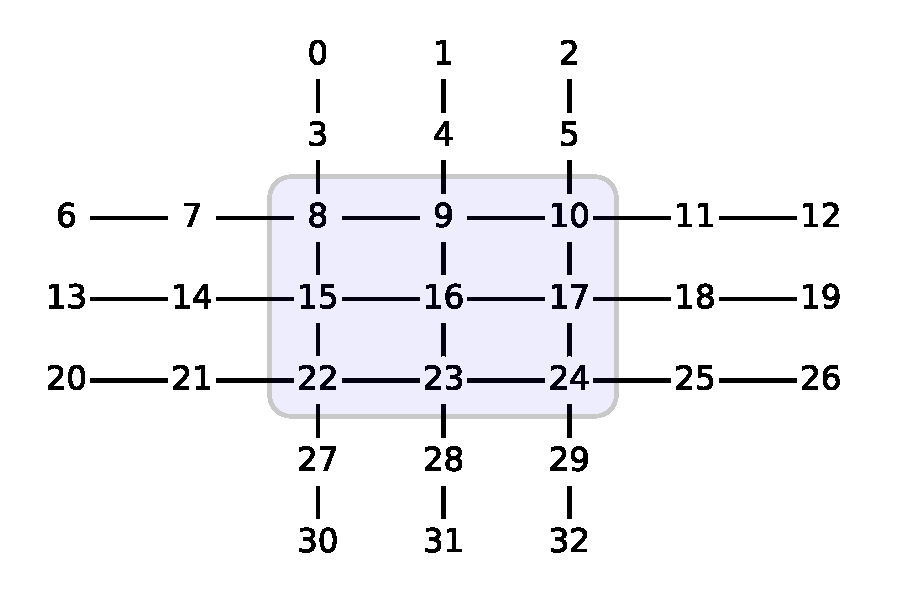
\includegraphics[width=0.29\linewidth]{web1center}
%  }
%  \hfill %\hspace{\figsep}
%  \subcaptionbox{$`a\in [\frac{37}{20},\frac{58}{25}){;}`b = 0.85$\label{fig:2web}}{ %3*9+4*6-12 / 48-9 = 27+12 / 41 = 39/41
%    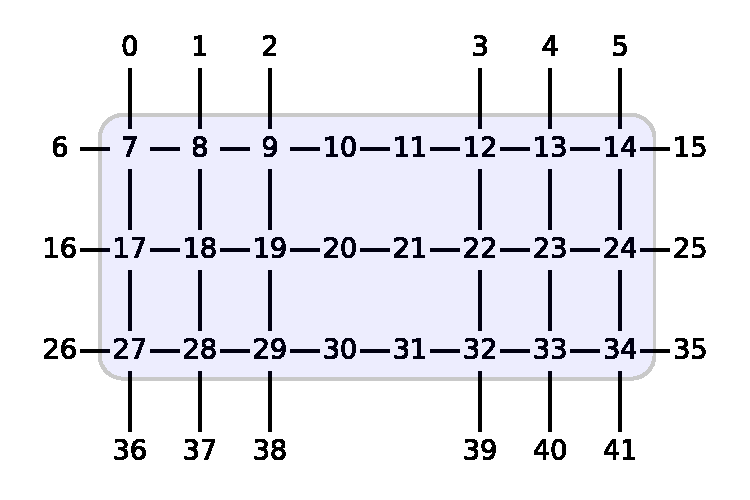
\includegraphics[width=0.3\linewidth]{web2center2}
%  }
%  \hfill %\hspace{\figsep}
%  \subcaptionbox{$`a\in [\frac{58}{25},\frac{75}{32}){;}`b = 0.85$\label{fig:2web2}}{ %3*9+4*6-12 / 48-9 = 27+12 / 41 = 39/41
%    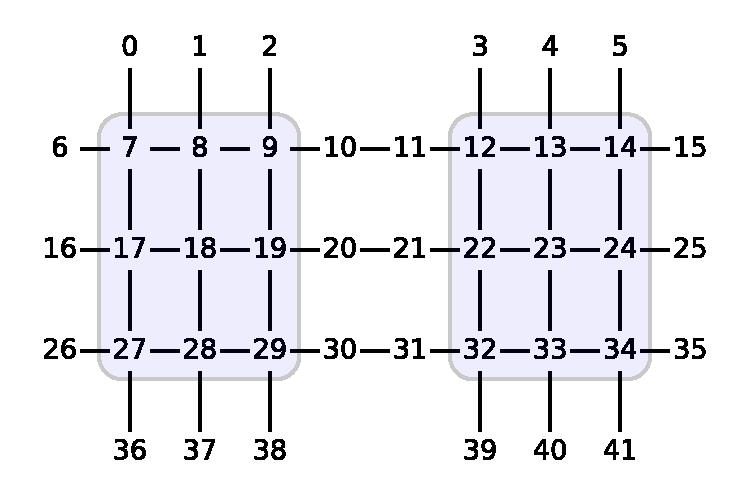
\includegraphics[width=0.3\linewidth]{web2center}
%  }
%  % \hspace{\figsep}
%  % \subcaptionbox{\label{fig:mweb}}{
%    
%  % }
%  \caption{Undirected web graphs with boxes showing web centers identified as $(`a,`b)$-communities for the range of $`a$ and $`b$ specified. There are no other $(`a,`b)$-communities except the entire set of nodes for $`a$ smaller than the specified range.}
%  \label{fig:web-center}
%\end{figure}
%
%\begin{figure}
%  \centering
%  \def\figsep{.4cm}
%  \def\dist{1}
%  \def\disty{.9}
%  \subcaptionbox{$`a\in [\frac{1}{8},\frac1{2})$\label{fig:1web-cc}}{
%    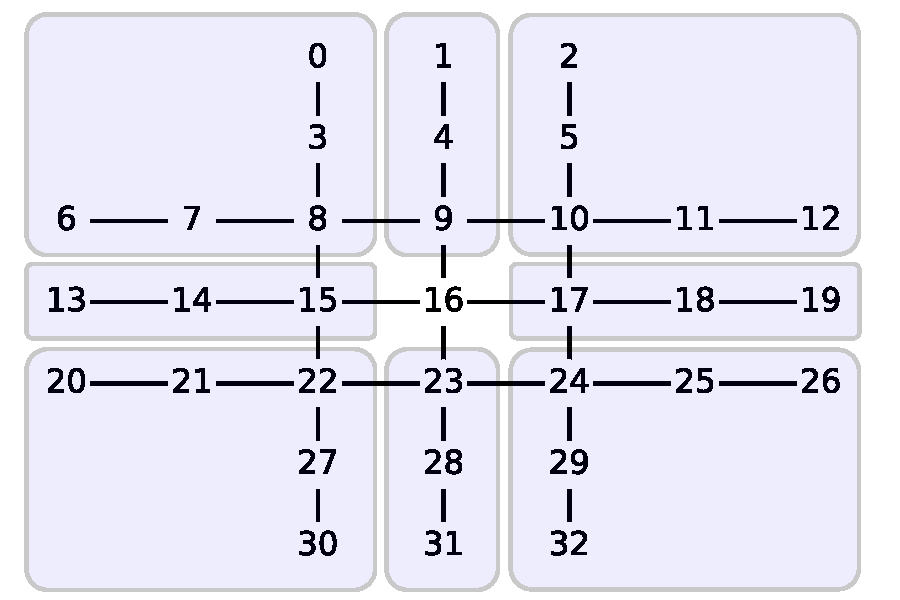
\includegraphics[width=0.3\linewidth]{web1peripheral}
%  }
%  \hfill %\hspace{\figsep}
%  \subcaptionbox{$`a\in [\frac1{2},1)$\label{fig:1web2-cc}}{% 
%    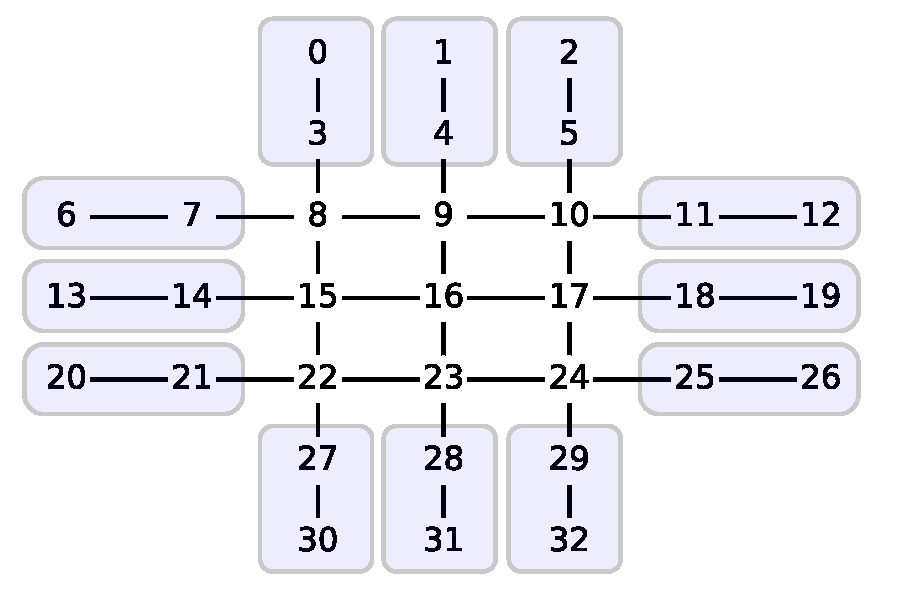
\includegraphics[width=0.3\linewidth]{web1peripheral2}
%  }
%  \hfill %\hspace{\figsep}
%  \subcaptionbox{$`a\in [\frac4{41},1)$\label{fig:2web-cc}}{% 
%    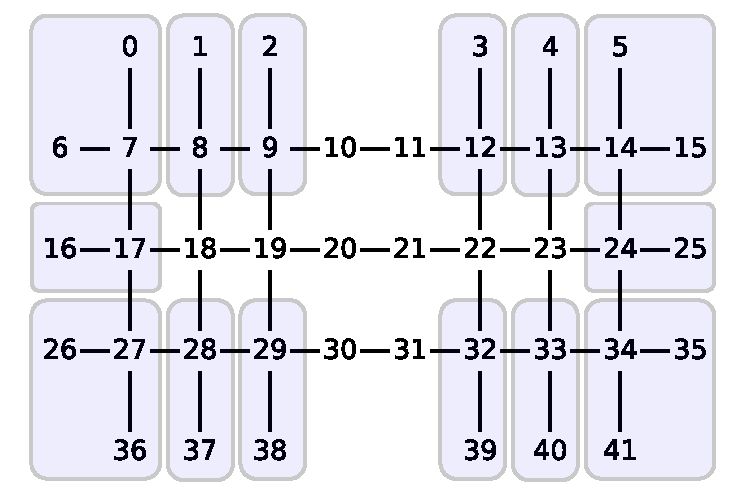
\includegraphics[width=0.3\linewidth]{web2peripheral}
%  }
%  % \hspace{\figsep}
%  % \subcaptionbox{\label{fig:mweb}}{
%    
%  % }
%  \caption{Boxes showing all the communities returned by cut-clustering within the given range of $`a$. The other communities returned are singletons for larger $`a$ and the entire set for smaller $`a$.}
%  \label{fig:web-peripheral}
%\end{figure}


\usetikzlibrary{arrows,patterns}

\pgfdeclarepatternformonly{soft crosshatch}{\pgfqpoint{-1pt}{-1pt}}{\pgfqpoint{4pt}{4pt}}{\pgfqpoint{3pt}{3pt}}%
{
  \pgfsetstrokecolor{blue}
  \pgfsetstrokeopacity{0.3}
  \pgfsetlinewidth{0.4pt}
  \pgfpathmoveto{\pgfqpoint{3.1pt}{0pt}}
  \pgfpathlineto{\pgfqpoint{0pt}{3.1pt}}
  \pgfpathmoveto{\pgfqpoint{0pt}{0pt}}
  \pgfpathlineto{\pgfqpoint{3.1pt}{3.1pt}}
  \pgfusepath{stroke}
}

\tikzstyle{cut}=[fill=red, fill opacity=0.2,rounded corners,inner sep=0.1em]
\tikzstyle{cluster}=[pattern=soft crosshatch, pattern color=blue, fill opacity=0.2,rounded corners,inner sep=0.1em]
\tikzstyle{v}=[circle,draw,fill=gray!40,minimum size=2,transform shape]
\tikzstyle{nodestyle}=[every node/.style={transform shape}]

\begin{figure}
\def\s{.3}
\centering
\subcaptionbox{\label{fig:oneweb-community}}{
\begin{tikzpicture}[scale=\s]
  \foreach \x in {0,...,6}
    \foreach \y in {0,...,2} 
       \node [v]  (a\x\y) at (\x,\y) {};

  \foreach \y in {0,...,2}
    \foreach \x [count=\xi] in {0,...,5}  
      \draw (a\x\y)--(a\xi\y);


  \foreach \x in {0,...,2}
    \foreach \y in {0,...,6} 
       \node [v]  (b\x\y) at (\x+2,\y-2) {};

  \foreach \x in {0,...,2}
    \foreach \y [count=\yi] in {0,...,5}  
      \draw (b\x\y)--(b\x\yi);

	\node[cluster,fit=(a20) (a42)] {};
\end{tikzpicture}
}
%
\subcaptionbox{\label{fig:oneweb-cut1}}{
\begin{tikzpicture}[scale=\s]
  \foreach \x in {0,...,6}
    \foreach \y in {0,...,2} 
       \node [v]  (a\x\y) at (\x,\y) {};

  \foreach \y in {0,...,2}
    \foreach \x [count=\xi] in {0,...,5}  
      \draw (a\x\y)--(a\xi\y);


  \foreach \x in {0,...,2}
    \foreach \y in {0,...,6} 
       \node [v]  (b\x\y) at (\x+2,\y-2) {};

  \foreach \x in {0,...,2}
    \foreach \y [count=\yi] in {0,...,5}  
      \draw (b\x\y)--(b\x\yi);

	\node[cut,fit=(a00) (b00)] {}; \node[cut,fit=(a62) (b26)] {};
	\node[cut,fit=(a02) (b06)] {}; \node[cut,fit=(a60) (b20)] {};
	\node[cut,fit=(a01) (a21)] {}; \node[cut,fit=(a41) (a61)] {};
	\node[cut,fit=(b10) (b12)] {}; \node[cut,fit=(b14) (b16)] {};
\end{tikzpicture}
}
%
\subcaptionbox{\label{fig:oneweb-cut2}}{
\begin{tikzpicture}[scale=\s]
  \foreach \x in {0,...,6}
    \foreach \y in {0,...,2} 
       \node [v]  (a\x\y) at (\x,\y) {};

  \foreach \y in {0,...,2}
    \foreach \x [count=\xi] in {0,...,5}  
      \draw (a\x\y)--(a\xi\y);


  \foreach \x in {0,...,2}
    \foreach \y in {0,...,6} 
       \node [v]  (b\x\y) at (\x+2,\y-2) {};

  \foreach \x in {0,...,2}
    \foreach \y [count=\yi] in {0,...,5}  
      \draw (b\x\y)--(b\x\yi);

	\node[cut,fit=(a00) (a10)] {}; \node[cut,fit=(a50) (a60)] {};
	\node[cut,fit=(a01) (a11)] {}; \node[cut,fit=(a51) (a61)] {};
	\node[cut,fit=(a02) (a12)] {}; \node[cut,fit=(a52) (a62)] {};
	\node[cut,fit=(b00) (b02)] {}; \node[cut,fit=(b04) (b06)] {};
	\node[cut,fit=(b10) (b12)] {}; \node[cut,fit=(b14) (b16)] {};
	\node[cut,fit=(b20) (b22)] {}; \node[cut,fit=(b24) (b26)] {};
\end{tikzpicture}
}
  \caption{
	  An example graph that exhibits a grid-like center that
	  connects to threads of nodes along the grid's perimeter. Communities and cut-clusters are
	  highlighted using a crosshatch (blue) and no-pattern (red) marks, respectively.
	  (a) Shows the returned community for $\alpha \in [\frac{31}{20},\frac{27}{16})$ and $\beta = 0.7$, and 
	  (b) the cut-clusters for $\alpha\in [\frac{1}{8},\frac{1}{2})$
	  and (c) the cut-clusters for $\alpha\in [\frac{1}{2}, 1)$.
	  There are no other non-trivial (i.e., the entire set) solutions.
  }
  \vspace{-1em}
  \label{fig:oneweb}
\end{figure}




\begin{figure}
\def\s{.28}
%\centering
\subcaptionbox{\label{fig:twowebs-community1}}{
\begin{tikzpicture}[scale=\s]
  \foreach \x in {0,...,9}
    \foreach \y in {0,...,2} 
       \node [v]  (a\x\y) at (\x,\y) {};

  \foreach \y in {0,...,2}
    \foreach \x [count=\xi] in {0,...,8}  
      \draw (a\x\y)--(a\xi\y);


  \foreach \x in {0,1,2, 5,6,7}
    \foreach \y in {0,...,4} 
       \node [v]  (b\x\y) at (\x+1,\y-1) {};

  \foreach \x in {0,1,2, 5,6,7}
    \foreach \y [count=\yi] in {0,...,3}  
      \draw (b\x\y)--(b\x\yi);

	\node[cluster,fit=(a10) (a82)] {};
\end{tikzpicture}
}
%
\subcaptionbox{\label{fig:twowebs-community2}}{
\begin{tikzpicture}[scale=\s]
  \foreach \x in {0,...,9}
    \foreach \y in {0,...,2} 
       \node [v]  (a\x\y) at (\x,\y) {};

  \foreach \y in {0,...,2}
    \foreach \x [count=\xi] in {0,...,8}  
      \draw (a\x\y)--(a\xi\y);


  \foreach \x in {0,1,2, 5,6,7}
    \foreach \y in {0,...,4} 
       \node [v]  (b\x\y) at (\x+1,\y-1) {};

  \foreach \x in {0,1,2, 5,6,7}
    \foreach \y [count=\yi] in {0,...,3}  
      \draw (b\x\y)--(b\x\yi);
%
	\node[cluster,fit=(a10) (a32)] {};
	\node[cluster,fit=(a60) (a82)] {};

\end{tikzpicture}
}
%
\subcaptionbox{\label{fig:twowebs-cut}}{
\begin{tikzpicture}[scale=\s]
  \foreach \x in {0,...,9}
    \foreach \y in {0,...,2} 
       \node [v]  (a\x\y) at (\x,\y) {};

  \foreach \y in {0,...,2}
    \foreach \x [count=\xi] in {0,...,8}  
      \draw (a\x\y)--(a\xi\y);


  \foreach \x in {0,1,2, 5,6,7}
    \foreach \y in {0,...,4} 
       \node [v]  (b\x\y) at (\x+1,\y-1) {};

  \foreach \x in {0,1,2, 5,6,7}
    \foreach \y [count=\yi] in {0,...,3}  
      \draw (b\x\y)--(b\x\yi);

	\node[cut,fit=(a00) (b00)] {}; \node[cut,fit=(a92) (b74)] {};
	\node[cut,fit=(a01) (a11)] {}; \node[cut,fit=(a91) (a81)] {};
	\node[cut,fit=(a02) (b04)] {}; \node[cut,fit=(a90) (b70)] {};

	\node[cut,fit=(b10) (b11)] {}; \node[cut,fit=(b13) (b14)] {};
	\node[cut,fit=(b20) (b21)] {}; \node[cut,fit=(b23) (b24)] {};
	\node[cut,fit=(b50) (b51)] {}; \node[cut,fit=(b53) (b54)] {};
	\node[cut,fit=(b60) (b61)] {}; \node[cut,fit=(b63) (b64)] {};
\end{tikzpicture}
}
  \caption{
	  %An example graph that resembles a spider's web in that it exhibits a grid-like center that
	  %connects to threads of nodes along the grid's perimeter.
	  Similar to Fig.~\ref{fig:oneweb}.
	  (a) Shows the returned community for $\alpha \in [\frac{37}{20},\frac{58}{25})$ and $\beta = 0.85$, 
	  (b) the communities for $\alpha\in [\frac{58}{25},\frac{75}{32})$ and $\beta = 0.85$,
	  and (c) the cut-clusters for $\alpha\in [\frac{4}{41}, 1)$.
	  There are no other, non-trivial, solutions.
  }
  \label{fig:twowebs}
\end{figure}


To illustrate the benefits of the proposed communities over cut-clustering for larger networks than
those in \figref{fig:eg12}, we implemented and tested both algorithms on the graphs in
Figs.~\ref{fig:oneweb} and \ref{fig:twowebs}. The graph in \figref{fig:oneweb} contains a grid-like center,
with peripheral-like chains of nodes attached to the grid's perimeter.
The graph in Fig.~\ref{fig:twowebs} is similarly constructed, but with two grid-like centers.
In both figures, it is desirable to differentiate the (denser) grid-like centers from the (sparser)
peripherals.
%centers, i.e., the peripherals of the webs consist of vertex disjoint chains. The goal is to detect
%the web centers as communities since they are the denser subgraphs.


The desired center is identified as a community in Fig.~\ref{fig:oneweb-community}, while
cut-clustering only returns undesirable solutions, Figs.~\ref{fig:oneweb-cut1} and
\ref{fig:oneweb-cut2}. (See the figure's caption for details.) 
Note that the desired center is not a web community since each of its four corner nodes does not
satisfy \eqref{eq:support-community}, which demonstrates the benefit of choosing $\beta > 0$.
This also explains the undesirable behaviour of cut-clustering since a cut-cluster allows at most
one of its members to violate \eqref{eq:support-community} \cite[Lemma~3.1]{flake:cut-clustering}.
(See \ifPAGELIMIT\cite[Appendix~A]{long} \else Appendix~\ref{sec:comparison-cut} \fi for more details.)
Similar observations can be made using Fig.~\ref{fig:twowebs}, where it is not hard to see that the
same issues extend to larger, and other types of, graphs.  More experimental results on synthetic
and real-world data sets can be found in
\ifPAGELIMIT\cite[Appendix~B]{long}.\else Appendix~\ref{sec:comparison-other}.\fi


%To illustrate the benefits of the proposed communities over cut-clustering for larger networks than those in \figref{fig:eg12}, we implemented and tested both algorithms on the graphs in \figref{fig:web-center}. Note that all the graphs in \figref{fig:web-center} contains web centers, each of which consist of nodes interconnected into $2$-by-$2$ grids. The nodes between different web centers, i.e., the peripherals of the webs consist of vertex disjoint chains. The goal is to detect the web centers as communities since they are the denser subgraphs.
%
%As indicated in \figref{fig:web-center}, all web centers are returned as communities when $`a$ and $`b$ are sufficiently large. In contrast, cut-clustering always fail to return the web centers regardless of the choice of $`a$. Instead, the peripherals are returned as shown in \figref{fig:1web-b}, \figref{fig:1web-c}. This is expected because, by \cite[Lemma~3.1]{flake:cut-clustering}, all but one node in a cut cluster must satisfy the condition~\eqref{eq:support-community}. Web centers cannot be cut clusters because their four corner points do not satisfy \eqref{eq:support-community}, e.g., Node 8 in the web center of \figref{fig:1web} and Node 12 in the web center of \figref{fig:2web} has the same number of internal and external edges. The experiments confirm that the internal support plays an important role in identifying the web centers as communities, and so our proposed solution can strictly improves over the previous solution. Following the same logic, it is not difficult to see that the same issue may arise regardless of the number of web centers or how far apart they are. The same problem can also arise in other types of graphs.
%

% Consider the web-spider graph in \figref{fig:web}, which is an undirected graph with edges of unit weight. Cut clustering returns only the four legs and their segments as communities but not the center four more interconnected nodes. (show ...) However, the center is a meaningful community and is returned as an $(`a,`b)$-community for (range of alpha and value of beta).

% \figref{} shows another example where there are more than one web centers. Again, our approach finds the web centers but cut-clustering only returns the leg segments instead of the web centers.

% \figref{} shows another example with more legs and a larger center. Indeed, the center is not a supporting community due to the many external connections to the legs. Again, our approach returns the center but cut-clustering does not. 
